\documentclass[12pt, titlepage]{article}

\usepackage{fullpage}
\usepackage[round]{natbib}
\usepackage{multirow}
\usepackage{booktabs}
\usepackage{tabularx}
\usepackage{graphicx}
\usepackage{float}
\usepackage{hyperref}
\hypersetup{
    colorlinks,
    citecolor=black,
    filecolor=black,
    linkcolor=red,
    urlcolor=blue
}
\usepackage[round]{natbib}

\newcounter{acnum}
\newcommand{\actheacnum}{AC\theacnum}
\newcommand{\acref}[1]{AC\ref{#1}}

\newcounter{ucnum}
\newcommand{\uctheucnum}{UC\theucnum}
\newcommand{\uref}[1]{UC\ref{#1}}

\newcounter{mnum}
\newcommand{\mthemnum}{M\themnum}
\newcommand{\mref}[1]{M\ref{#1}}

\title{SE 3XA3: Module Guide\\SnakeGame Project}

\author{ Team L03G09
		\\ Qiang Gao  (gaoq20)
		\\ Zhiwei Li  (liz342)
		\\ Longwei Ye (yel16)
}

\date{\today}

\begin{document}

\maketitle

\pagenumbering{roman}
\tableofcontents
\listoftables
\listoffigures

\begin{table}[bp]
\begin{tabularx}{\textwidth}{p{3cm}p{2cm}X}
\toprule {\bf Date} & {\bf Version} & {\bf Notes}\\
\midrule
2022/3/15 & 1.0 & Complete Section 1, 2\\
2022/3/16 & 1.1 & Complete Section 3\\
2022/3/17 & 1.2 & Complete Section 4, 5\\
2022/3/18 & 1.3 & Complete Section 6, 7, 8\\
2022/3/18 & 1.4 & Revise MG Document\\
\bottomrule
\end{tabularx}
\caption{\bf Revision History}
\end{table}

\newpage

\pagenumbering{arabic}

\section{Introduction}
\subsection{Overview of the Project}
The SnakeGame is a re-implementation of the open-source game that allows the user to cutomize and control the ``snake'', and gain points by eating the blocks on the gameboard.

\subsection{Context}
This document is the Module Guide(MG), which is based on the previous Software Requirements Specification document(SRS). The purpose of the MG document is to establish a modular break-down of the project and to show the project's structure. Besides, as the SRS document defines the functional and non-functional requirements of the project, MG should document how the system meets the requirements defined in SRS.\\

\noindent In addition to MG, the Module Interface Specification(MIS) is also documented, which specifies the external details(state and environment variables, Assumptions, Access Program Semantics, Inputs, Outputs, Exceptions) of the module, which provides a further view of how the project is implemented.

\subsection{Design Principles}
As MG is showing the decomposition of the system into modular subsystems, this is accomplished following the design principle of Information Hiding and Encapsulation. Besides, the Use Hierarchy between modules should follow the principle of High Cohesion, Low Coupling.\\

\noindent To be more specific, the principle of information hiding states that each module hides a secret and the implementation of encapsulation is when the information is changing, this information is performed in the module and the information becomes the secret of it. Last but not least, High cohesion means that the functions within a module has a strong relation, whereas the relation between modules are tight, which is principle of low coupling.


\subsection{Document Structure}
The structure of the document are listed at the following:
\begin{itemize}
    \item \hyperref[SecChange]{Section 2} lists the anticipated and unlikely changes of the program's implementation. The listed items are used in the \hyperref[SecTM]{Traceability Matrix} section.
    \item \hyperref[SecMH]{Section 3} shows the details (modules and their secrets) of the module hierarchy.
    \item \hyperref[SecConnection]{Section 4} demonstrates the close relationship between SRS and MG by showing their connections.
    \item \hyperref[SecMD]{Section 5} gives the details of the decomposed modules of the system, including:
    \begin{itemize}
        \item Module Name
        \item Secrets
        \item Services
        \item Responsibility
    \end{itemize}
    \item \hyperref[SecTM]{Section 6} provides the Traceability Matrix, showing the connection between requirements in SRS and the modules, as well the relationship between Anticipated Changes and the modules.
    \item \hyperref[SecUse]{Section 7} is the Use Hierarchy between modules.
    \item \hyperref[SecPS]{Section 8} lists the project schedule.
\end{itemize}

\subsubsection{Naming Conversion and Terminology}
\begin{table}[!htbp]
\begin{tabularx}{\textwidth}{p{4cm}p{9cm}X}
\toprule {\bf Terms} & {\bf Definitions}\\
\midrule
SRS & Software Requirements Specification\\
MG & Module Guide\\
MIS & Module Internal Specification\\
JavaScript &  A programming language used to implement core script for World Wide Web\\
BGM & Background Music\\
N/I & Not Implemented\\
\bottomrule
\end{tabularx}
\caption{\bf Definitions}
\label{TblD}
\end{table}


\section{Anticipated and Unlikely Changes} \label{SecChange}

This section lists possible changes to the system. According to the likeliness
of the change, the possible changes are classified into two
categories. Anticipated changes are listed in Section \ref{SecAchange}, and
unlikely changes are listed in Section \ref{SecUchange}.

\subsection{Anticipated Changes} \label{SecAchange}

Anticipated changes are the source of the information that is to be hidden
inside the modules. Ideally, changing one of the anticipated changes will only
require changing the one module that hides the associated decision. The approach
adapted here is called design for
change.

\begin{description}
\item[\refstepcounter{acnum} \actheacnum \label{acHardware}:] The specific
  hardware on which the software is running.
\item[\refstepcounter{acnum} \actheacnum \label{acGUI}:] The graphical user interface elements used to retrieve user input and their format.
\item[\refstepcounter{acnum} \actheacnum \label{acFucntion}:] Additional functionality or mechanism for the game.
\item[\refstepcounter{acnum} \actheacnum \label{acOutput}:] The format of the output data.

\end{description}

\subsection{Unlikely Changes} \label{SecUchange}

The module design should be as general as possible. However, a general system is
more complex. Sometimes this complexity is not necessary. Fixing some design
decisions at the system architecture stage can simplify the software design. If
these decision should later need to be changed, then many parts of the design
will potentially need to be modified. Hence, it is not intended that these
decisions will be changed.

\begin{description}
\item[\refstepcounter{ucnum} \uctheucnum \label{ucIO}:] Input/Output devices
  (Input: File and Keyboard, Output: File, Memory, and Screen).
\item[\refstepcounter{ucnum} \uctheucnum \label{ucO}:] The original mechanism of the game.
\item[\refstepcounter{ucnum} \uctheucnum \label{ucG}:] The Graph of nodes that represents the playable grid.
\item[\refstepcounter{ucnum} \uctheucnum \label{ucS}:] There will always be
  a source of input data external to the software.
\item[\refstepcounter{ucnum} \uctheucnum \label{ucF}:]
The format of the input data.
\item[\refstepcounter{ucnum} \uctheucnum \label{ucDeafault}:]
Default settings for input.
\end{description}

\section{Module Hierarchy} \label{SecMH}

This section provides an overview of the module design. Modules are summarized
in a hierarchy decomposed by secrets in Table \ref{TblMH}. The modules listed
below, which are leaves in the hierarchy tree, are the modules that will
actually be implemented.

\begin{description}
\item [\refstepcounter{mnum} \mthemnum \label{mHH}:] Hardware-Hiding Module
\item [\refstepcounter{mnum} \mthemnum \label{mV}:] View Module
\item [\refstepcounter{mnum} \mthemnum \label{mBC}:] BGM Control Module
\item [\refstepcounter{mnum} \mthemnum \label{mIC}:] Inputs Checking Module
\item [\refstepcounter{mnum} \mthemnum \label{mGC}:] Game Control Module
\item [\refstepcounter{mnum} \mthemnum \label{mS}:] SnakeGame Module
\item [\refstepcounter{mnum} \mthemnum \label{mH}:] History Module
\item [\refstepcounter{mnum} \mthemnum \label{mSC}:] Snake Color Module
\end{description}


\begin{table}[h!]
\centering
\begin{tabular}{p{0.3\textwidth} p{0.6\textwidth}}
\toprule
\textbf{Level 1} & \textbf{Level 2}\\
\midrule

{Hardware-Hiding Module} & ~ \\
\midrule

\multirow{7}{0.3\textwidth}{Behaviour-Hiding Module} & View Module\\
& BGM Control Module\\
& Inputs Checking Module\\
& Game Control Module\\
\midrule

\multirow{3}{0.3\textwidth}{Software Decision Module} & SnakeGame Module\\
& History Module\\
& Snake Color Module\\
\bottomrule

\end{tabular}
\caption{\textbf{Module Hierarchy}}
\label{TblMH}
\end{table}


\section{Connection Between Requirements and Design} \label{SecConnection}

The system is intended to satisfy all of the functional and non-functional requirements that were initially specified in the SRS. At this stage, in order to meet information hiding principle as well as low coupling and high cohesion, we decomposed the system into modules, assign responsibilities to those modules and ensure that they fit together to achieve our global goals. The connection
between requirements and modules is listed in Table \ref{TblRT}. Section 5 specifies how we decomposed the modules.

\section{Module Decomposition} \label{SecMD}

Modules are decomposed according to the principle of ``information hiding''
proposed by \citet{ParnasEtAl1984}. The \emph{Secrets} field in a module
decomposition is a brief statement of the design decision hidden by the
module. The \emph{Services} field specifies \emph{what} the module will do
without documenting \emph{how} to do it. For each module, a suggestion for the
implementing software is given under the \emph{Implemented By} title. If the
entry is \emph{OS}, this means that the module is provided by the operating
system or by standard programming language libraries.  Also indicate if the
module will be implemented specifically for the software.

Only the leaf modules in the
hierarchy have to be implemented. If a dash (\emph{--}) is shown, this means
that the module is not a leaf and will not have to be implemented. Whether or
not this module is implemented depends on the programming language
selected.

\subsection{Hardware Hiding Modules (\mref{mHH})}
\begin{description}
\item[Secrets:]The data structure and algorithm used to implement the virtual
  hardware.
\item[Services:] This module serves as a virtual hardware used by the rest part of the system, which allows the system to implements actions such as display outputs and accept inputs from the user.
\item[Implemented By:] OS
\end{description}

\subsection{Behaviour-Hiding Module}
\begin{description}
\item[Secrets:]The contents of the required behaviours.
\item[Services:]This module serves as the connector between the Hardware Hiding Modules and the Software Decision Module, which describes the externally visible behaviour of the system listed in the SRS document.
\item[Implemented By:] N/A
\end{description}

\subsubsection{View Module (\mref{mV})}
\begin{description}
\item[Secrets:] GUI.
\item[Services:] Allows the user to see the game components and to interact with the game.
\item[Implemented By:]HTML
\end{description}

\subsubsection{BGM Control Module (\mref{mBC})}
\begin{description}
\item[Secrets:] BGM and volume control
\item[Services:] Allows the user to play/pause the BGM and also to change the BGM's playing volume.
\item[Implemented By:]JavaScript
\end{description}

\subsubsection{Inputs Checking Module (\mref{mIC})}
\begin{description}
\item[Secrets:] Inputs
\item[Services:] Allows the user to specify valid snake's color and username.
\item[Implemented By:] JavaScript
\end{description}

\subsubsection{Game Control Module (\mref{mGC})}
\begin{description}
\item[Secrets:] Game control algorithm
\item[Services:] Accepts user inputs and updates the game status.
\item[Implemented By:]JavaScript
\end{description}


\subsection{Software Decision Module}
\begin{description}
\item[Secrets:] Data Structures and the secrets of the module that are \emph{not} discussed in the SRS document.
\item[Services:] Includes data structure and algorithms used in the system that
  do not provide direct interaction with the user. 
  % Changes in these modules are more likely to be motivated by a desire to
  % improve performance than by externally imposed changes.
\item[Implemented By:] N/A
\end{description}

\subsubsection{SnakeGame Module (\mref{mS})}
\begin{description}
\item[Secrets:]SnakeGame objects
\item[Services:]Stores the in-game elements status(i.e. position of the snake and supplements, speed of the snake, points that the user has gained.)
\item[Implemented By:]JavaScript
\end{description}

\subsubsection{History Module (\mref{mH})}
\begin{description}
\item[Secrets:]Array
\item[Services:]Stores the previous game history(player name and score.)
\item[Implemented By:]JavaScript
\end{description}

\subsubsection{Snake Color Module (\mref{mSC})}
\begin{description}
\item[Secrets:]Color of the snake
\item[Services:]Stores the color specification of the snake.
\item[Implemented By:]JavaScript
\end{description}

\section{Traceability Matrix} \label{SecTM}
% the table should use mref, the requirements should be named, use something
% like fref
\begin{table}[H]
\centering
\begin{tabular}{p{0.2\textwidth} p{0.6\textwidth}}
\toprule
\textbf{Req.} & \textbf{Modules}\\
\midrule
R1 & \mref{mV}, \mref{mIC}, \mref{mGC}, \mref{mS}, \mref{mSC}\\
R2 & \mref{mV}, \mref{mIC}, \mref{mGC}\\
R3 & N/I\\
R4 & \mref{mV}, \mref{mGC}, \mref{mH}\\
R5 & \mref{mV}\\
R6 & \mref{mV}\\
R7 & N/I\\
R8 & \mref{mGC}, \mref{mS}\\
R9 & \mref{mS}, \mref{mHH}\\
R10 & \mref{mS}\\
R11 & \mref{mS}\\
R12 & \mref{mS}\\
R13 & \mref{mV}, \mref{mS}\\
R14 & \mref{mGC}\\
R15 & \mref{mGC}, \mref{mH}\\
R16 & \mref{mS}\\
R17 & N/I\\
R18 & \mref{mS}\\
\bottomrule
\end{tabular}
\caption{\textbf{Trace Between Requirements and Modules}}
\label{TblRT}
\end{table}

\begin{table}[H]
\centering
\begin{tabular}{p{0.2\textwidth} p{0.6\textwidth}}
\toprule
\textbf{AC} & \textbf{Modules}\\
\midrule
\acref{acHardware} & \mref{mHH}\\
\acref{acGUI} & \mref{mV}, \mref{mGC}, \mref{mIC}, \mref{mS}\\
\acref{acFucntion} & \mref{mS}, \mref{mGC}\\
\acref{acOutput} & \mref{mS}\\
\bottomrule
\end{tabular}
\caption{\textbf{Trace Between Anticipated Changes and Modules}}
\label{TblACT}
\end{table}

\section{Use Hierarchy Between Modules} \label{SecUse}
\begin{figure}[H]
\centering
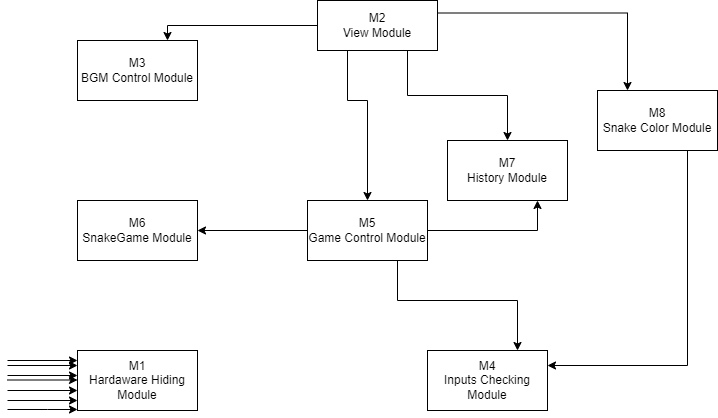
\includegraphics[width=1.0\textwidth]{./Figures/UHBM.png}
\caption{\textbf{Use hierarchy among modules}}
\label{FigUH}
\end{figure}

\section{Project Schedule} \label{SecPS}
\begin{figure}[H]
\centering
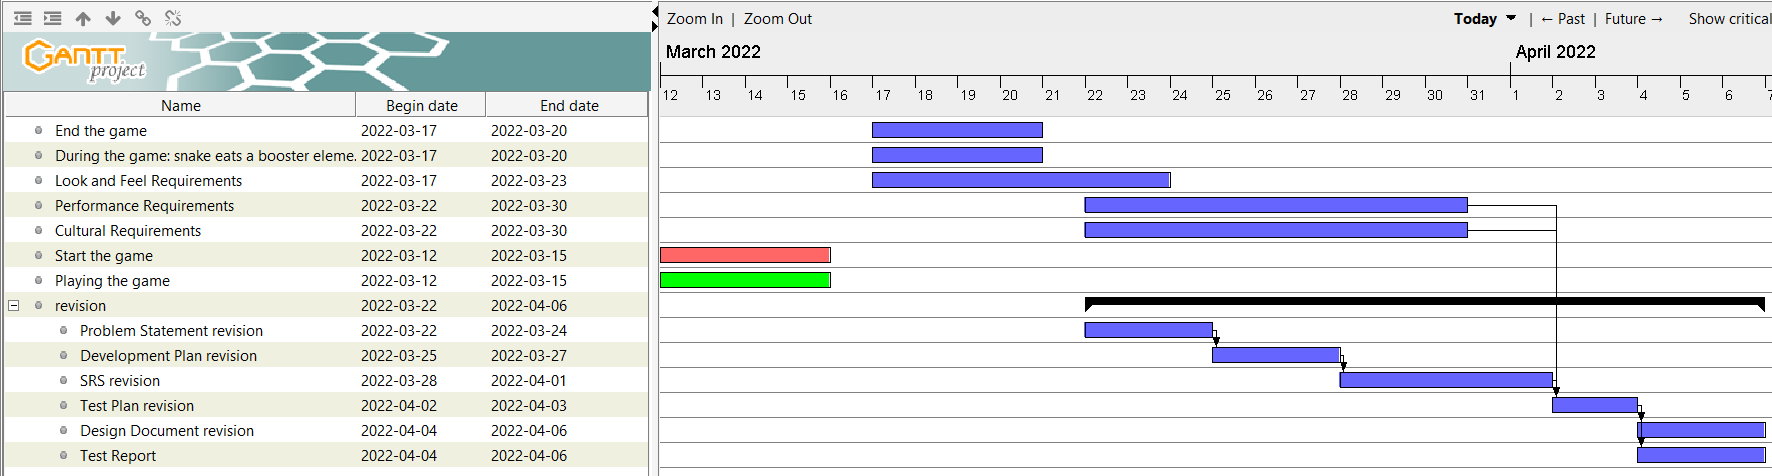
\includegraphics[width=1.0\textwidth]{./Figures/gantt.png}
\caption{\textbf{Time schedule}}
\label{FigUH}
\end{figure}

\begin{figure}[H]
\centering
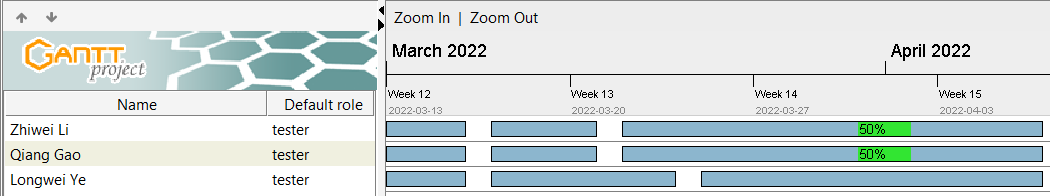
\includegraphics[width=1.0\textwidth]{./Figures/Resources.png}
\caption{\textbf{Resource divide}}
\label{FigUH}
\end{figure}
%\section*{References}

\bibliographystyle {plainnat}
\bibliography {MG}

\end{document}
